% \section{Introduction}
% \label{sec:intro} 
% Large language models (LLMs) have become essential for a broad spectrum of modern applications, ranging from digital assistants and document summarization to code and content creation\,\cite{apple_intelligence, gemini}. Their integration into organizational workflows has boosted user assistance and productivity in various scenarios\,\cite{whatsapp, apple_intelligence, gemini}, while also disrupting fields such as economics\,\cite{korinek2023generative}, research\,\cite{deep_research}, education\,\cite{lo2023impact}, and healthcare\,\cite{mesko2023imperative}. Despite producing fluent, context-aware outputs, LLMs typically demand substantial memory\,\cite{alizadeh2024llm}, compute\,\cite{grattafiori2024llama}, and training time\,\cite{jiang2024megascale}, incurring high deployment costs. Furthermore, concerns about data privacy\,\cite{llm_real_world_use_cases, yao2024survey} make local deployment on smartphones, laptops, or desktops particularly challenging. Smaller LLM variants (SLMs)\,\cite{meta_llama2_13b, mistral_7b, tii_falcon_7b} can reduce some computational burdens, but they often suffer from hallucinations\,\cite{sheng2023flexgenhighthroughputgenerativeinference} and cannot seamlessly incorporate fresh, user-specific data\,\cite{godey2024smalllanguagemodelsunderperform, knowledge1, knowledge2}. Offloading personal information to remote servers for content augmentation also raises serious privacy issues\,\cite{yao2024survey}.

% % \begin{figure}[t]
% %     \centering
% %     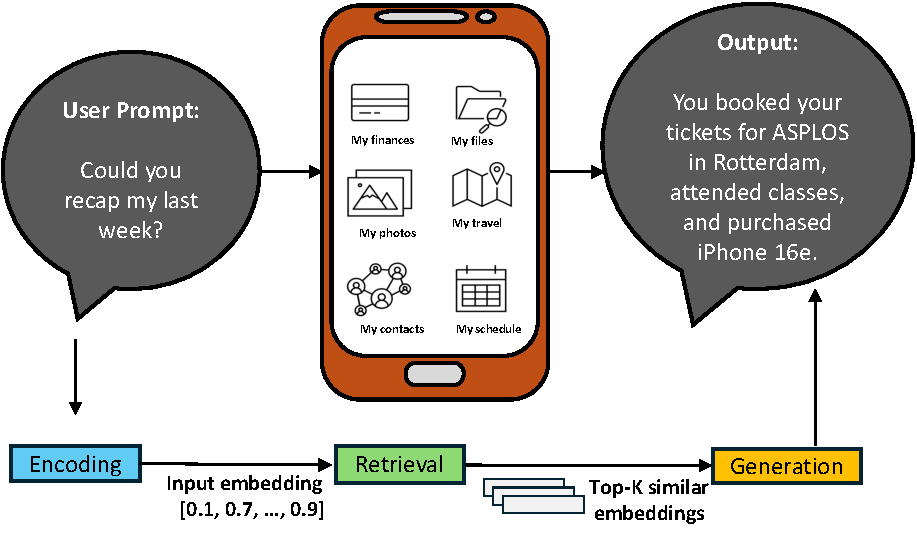
\includegraphics[width=0.75\linewidth]{Figs/personalized_need_for_GenAI.pdf}
% %     \caption{Toy deployment of RAG deployed on a mobile phone answering personalized questions.
% %     %answering grounded in the user's own history.
% %     }
% %     \label{fig:personalized_need_for_GenAI}
% %     %\vspace{-0.3in}
% % \end{figure}

% Retrieval-Augmented Generation (RAG) addresses these limitations by decoupling the knowledge store from the core language model, letting the system retrieve relevant passages from a local database and feed them into a smaller LLM\,\cite{meta_llama2_13b, mistral_7b, tii_falcon_7b}. When RAG is deployed locally, it offers personalized responses without retraining for new information. 
% %Because knowledge is stored externally (\cyan{in storage, }rather than fused into model parameters \cyan{which stay active in memory}), RAG can rely on compact generation models that better fit resource-constrained hardware. 
% Since knowledge is maintained externally (in storage) rather than embedded within the model's parameters (which reside in active memory), RAG can leverage smaller generation models that are more suitable for resource-limited hardware.
% % This type of design paves the way for on-device personal assistants, real-time analytics, or local chatbots that incorporate user-specific data. As on-device AI is projected to exceed \$125\,billion by 2032~\cite{mobile_ai_market}, RAG deployments present a promising avenue to deliver context-aware services within tight power and memory limits.
% This architectural approach enables applications such as on-device personal assistants, real-time analytics, and local chatbots that can integrate user-specific data. With the on-device AI market expected to surpass \$125\,billion by 2032~\cite{mobile_ai_market}, RAG-based solutions offer a compelling path toward delivering context-aware services under stringent power and memory constraints.


% %However, the deployment of RAG on edge \cyan{we bring edge here abruptly - let us define edge here.} devices presents non-trivial challenges. 
% A typical RAG pipeline entails: 
% \emph{(i)}~\textit{encoding} the user prompt into high-dimensional embeddings; 
% \emph{(ii)}~\textit{retrieving} \topk passages through a similarity search in local storage;
% \emph{(iii)}~\textit{augmenting} the retrieved data with the original prompt; and 
% \emph{(iv)}~\textit{generating} a final response using an LLM. 
% %Classically GPUs perform encoding and generation, while the CPU generally performs retrieval and prompt assembly.
% Traditionally, RAG pipelines split computation across heterogeneous resources: GPUs handle encoding and generation, while CPUs manage retrieval and prompt construction/augmentation ~\cite{jiang2024piperag, jin2024flashrag, rag_neurips, rago}. 
% This division introduces several inefficiencies, including frequent CPU--GPU data transfers~\cite{jin2024flashrag, jiang2024piperag}, repeated model load and unload cycles~\cite{jin2024flashrag}, and prolonged CPU idle periods, all of which inflate system-level data movement and reduce overall utilization. 
% While unified memory can alleviate some of these transfers~\cite{EdgeRAG}, key bottlenecks persist: limited memory capacity, constrained interconnect bandwidth, and rigid vectorization support often restrict end-to-end throughput. 
% Coordinating GPU kernels for encoding and generation with concurrent CPU-driven retrieval threads further compounds the challenge, particularly under dynamic workloads that require simultaneously low latency and high throughput.

% %%%% BKP %%%%
% % Traditionally, encoding and generation tasks are handled by GPUs, whereas retrieval and prompt construction are typically managed by the CPU~\cite{jiang2024piperag, jin2024flashrag, rag_neurips, rago}.
% % This bifurcated approach triggers frequent CPU--GPU transfers~\cite{jin2024flashrag, jiang2024piperag}, frequent model load/unload cycles~\cite{jin2024flashrag}, and significant CPU idle time, diminishing overall utilization, and inflating system-level data-transfer overheads. \textcolor{violet}{
% % Although having unified memory can partially mitigate data movement~\cite{EdgeRAG}, other critical bottlenecks such as tighter memory budgets, narrower interconnects, and less flexible vectorization support
% % remain significant, often limiting end-to-end system throughput. 
% % %These limitations make repeated retrieval and model execution costly, motivating caching and the reuse of intermediate results to achieve consistent latency and higher overall efficiency across diverse hardware platforms.
% % }
% % %{Although having unified memory can partially mitigate data movement~\cite{EdgeRAG},
% % %edge platforms face additional 
% % %other critical bottlenecks such as tighter memory budgets, narrower interconnects, and less flexible vectorization support. 
% % Orchestrating GPU kernels for encoding/generation alongside CPU-based retrieval threads becomes even more complex, especially under workload variations that demand both low latency and high throughput.
% %%%% %%%% %%%%

% % \red{Several efforts have aimed to optimize RAG pipelines~\cite{jin2024ragcache, chan2024don, lin2025telerag, xu2024generative, finardi2024chronicles, quinn2024accelerating, jin2024flashrag, jiang2024piperag}, but most are designed for server-scale deployments and rely heavily on large, high-end GPUs. 
% % FlashRAG~\cite{jin2024flashrag}, for instance, adopts a modular architecture but assumes abundant GPU capacity, dedicating little attention to fine-grained CPU--GPU coordination. 
% % Similarly, PipeRAG~\cite{jiang2024piperag} mitigates GPU memory pressure via pipelining but still depends primarily on GPUs for encoding and performs only coarse CPU--GPU partitioning.  
% % EdgeRAG~\cite{EdgeRAG}, while targeting the NVIDIA Jetson~\cite{nvidia_jetson_orin} platform, focuses on on-demand embedding and does not provide a detailed quantitative analysis of memory, storage, compute and power constraints. 
% % Importantly, all of these works overlook the systematic orchestration of CPU resources, missing an opportunity to balance workloads aross available compute resources.
% % \textbf{Taken together, existing RAG optimization strategies largely fail to exploit the CPU’s potential and remain unsuitable for small-scale devices, where GPU resources are scarce and underutilization of CPU compute cycles severely degrades system efficiency.}}

% % \red{Curretly, RAG systems are increasingly being deployed on consumer-grade, resource-constrained personal compute devices such as laptops, desktops, smartphones, and kiosks for emerging applications such as personalized virtual assistants, local context-aware chatbots, real-time document summarization, and on-device analytics. Unlike datacenter servers, these devices operate under tighter compute, memory, and power budgets, and are further constrained by limited I/O and memory bandwidth. Such constraints exacerbate the challenges of efficiently orchestrating RAG workloads on edge hardware. Running these applications on-device avoids the latency, privacy risks, and connectivity dependence associated with cloud-based solutions, making edge deployments not just attractive but often necessary.}

% % \red{However, existing solutions face significant challenges in these settings. Most approaches prioritize GPU optimizations, relegating CPUs to I/O and memory-bound tasks, often leaving valuable CPU compute cycles underutilized. These challenges are compounded by the fact that consumer-grade edge devices typically house only a single accelerator (GPU, NPU, or similar). When both the encoding and generation stages compete for the same accelerator in a pipelined fashion, structural hazards arise: only one stage can run at a time, resulting in idle bubbles and wasted resources. With such stringent compute, memory, and bandwidth constraints, careful orchestration of RAG stages becomes critical. Conventional RAG staging strategies, designed with abundant resources in mind, often fail to accommodate the nuanced scheduling requirements of edge devices while meeting tighter Service Level Objectives (SLOs).}

% % \noindent\textbf{Open Problems and Our Focus:} \red{Deploying RAG pipelines effectively on consumer-grade edge devices raises several key questions. First, how can we balance CPU and GPU workloads to reduce idle resources and minimize costly data movement? Second, how can a single RAG pipeline adapt to vastly different objectives (e.g., latency-critical personal assistants vs. high-throughput local summarization) while operating under tight accelerator memory constraints? Third, how can we overcome the pipeline bubbles caused by structural hazards, where encoding and generation compete for the same accelerator? Finally, how can these orchestration strategies generalize across diverse hardware configurations, ensuring that resource-limited edge devices are able to meet strict performance and SLO targets? Existing approaches lack the \emph{stage-level orchestration} required to fully utilize multicore CPUs and mitigate structural hazards, leading to underutilized resources and degraded performance. Our focus is on defining and addressing these challenges, laying the foundation for fine-grained orchestration that unlocks efficient RAG execution on consumer-grade edge platforms.}


% Several efforts have aimed to optimize RAG pipelines~\cite{jin2024ragcache, chan2024don, lin2025telerag, xu2024generative, finardi2024chronicles, quinn2024accelerating, jin2024flashrag, jiang2024piperag}, where  
% most of these designs are targeted for server-scale deployments and rely heavily on large, high-end GPUs. 
% FlashRAG~\cite{jin2024flashrag}, for instance, adopts a modular architecture but assumes abundant GPU capacity, dedicating little attention to fine-grained CPU--GPU coordination. 
% Similarly, PipeRAG~\cite{jiang2024piperag} mitigates GPU memory pressure via pipelining, but still depends on GPUs for encoding and performs only coarse CPU--GPU partitioning.  To our knowledge, 
% EdgeRAG~\cite{EdgeRAG} is the first effort that targets RAG deployment on smaller devices (NVIDIA Jetson~\cite{nvidia_jetson_orin} platform). However, it uses on-demand embedding and does not consider a systematic CPU--GPU orchestration for effectively utilizing the limited compute and memory resources of Jetson.

% %a detailed quantitative analysis of memory, storage, compute, and power constraints.  
% %\textbf{Overall, existing RAG optimization strategies assume access to multiple A100/H100-class GPUs and abundant host resources, overlooking systematic CPU orchestration and leaving CPU compute cycles significantly underutilized.} 



% As RAG systems are increasingly deployed on consumer-grade, resource-constrained personal computing devices (or edge devices; e.g., laptops~\cite{desktop9}, desktops~\cite{desktop11, desktop10}, smartphones~\cite{mobile1, mobile1, mobile5}) for applications such as personalized virtual assistants, local chatbots, real-time document summarization, and on-device analytics, efficient deployment of RAGs on such platforms is an area of research that has been little explored. 
% Unlike datacenters, these devices operate under tighter compute, memory, and power budgets and are further constrained by limited I/O and memory bandwidth~\cite{nvidia_jetson_orin}.  
% They typically house only a single accelerator (GPU, NPU, or similar), forcing both the encoding and generation stages to compete for the same device. 
% This competition leads to \emph{structural hazards}, where only one stage can run at a time, causing pipeline bubbles and resource underutilization.  
% %Because conventional RAG staging strategies were designed assuming abundant resources, they struggle to accommodate these constraints, often prioritizing GPU optimizations while relegating CPUs to lightweight I/O tasks. 
% %The result is severe underutilization of multicore CPUs, inefficient accelerator usage, and degraded overall performance in edge settings. 


% \noindent\textbf{Problems in deploying RAG on edge platforms:}
% Deploying RAG pipelines effectively on consumer-grade edge devices raises several key questions. 
% First, how can we effectively use both the availbale CPUs and a GPU to balance pipelined RAG computation for reducing idle resources and minimizing costly data movement?  
% Second, how can a single RAG pipeline adapt to vastly different objectives (e.g., latency-critical personal assistants vs.\ high-throughput local summarization) while operating under tight accelerator memory constraints?  
% Third, how can we mitigate pipeline bubbles caused by structural hazards when encoding and generation share the same accelerator? 
% Fourth, can we exploit know architectural techniques such as caching for enhancing system level performance? 
% Finally, how can orchestration strategies generalize across diverse hardware configurations to meet strict performance and SLO targets?
% %\red{
% %Existing approaches lack the \emph{stage-level orchestration} required to fully leverage multicore CPUs and overcome these structural hazards, leaving valuable compute resources untapped. 
% %Our focus is on defining and addressing these challenges, laying the foundation for fine-grained orchestration that unlocks efficient RAG execution on consumer-grade edge platforms.
% %}
% %

% \noindent\textbf{Our Approach and Novelty:} 
% We present \textbf{MaestroRAG}, a new hardware-aware and model-agnostic RAG pipeline framework explicitly designed for \emph{consumer-grade edge devices}, which operate under tight compute, memory, and power budgets and typically feature only a single accelerator. 
% Unlike prior works that target accelerator-rich datacenter servers, MaestroRAG addresses the unique orchestration challenges of edge devices through fine-grained stage-level CPU--GPU coordination. 

% We begin by performing a detailed profiling of the RAG pipeline (Encoding, Retrieval,  Augmentation, Generation) to uncover key performance bottlenecks. This analysis reveals that (1) encoding and generation stages compete for limited GPU resources, creating a \emph{structural pipeline hazard}, (2) encoding is compute-bound and can be efficiently parallelized across multiple CPU cores for small batch sizes, and (3) retrieval/augmentation is memory-bound and often leaves CPUs underutilized. Building on these insights, MaestroRAG strategically offloads the encoding and retrieval stages to modern vectorized CPUs, removing GPU contention and increasing overall utilization.

% Our pipelined approach is paired with an adaptive batching strategy that handles both bursty queries and large batches, along with targeted software optimizations, like , opportunistic caching, memory-mapped indices, a shared encoder, and asynchronous multi-worker execution, to minimize query latency and maximize throughput. 
% \textbf{To the best of our knowledge, MaestroRAG is the first RAG pipeline framework that enables fine-grained CPU--GPU orchestration for this class of edge devices}, achieving performance gains that baseline datacenter-oriented solutions fail to deliver, while remaining agnostic to the choice of underlying encoder and LLM models.  
% Our work makes the following {\bf contributions}:

% % %%%%%%%%%%%%%%%%%%%% DR DAS ADDDED THIS %%%%%%%%%%%%%%%%%%%%
% % \noindent\textbf{Our Approach:} We propose a new pipeline framework, called MaestroRAG
% % %\footnote{Given the orchestration of the RAG stages on the heterogeneous platform, we title our work as \design{}.}
% % \emph{, explicitly designed} for edge deployments. First, we conduct a detailed system-level characterization to understand the overheads of the encoding, retrieval, augmentation, and generation stages in a RAG workflow. Building on these insights, we propose a three-stage pipeline -- Encode, Retrieval, and Generation -- where each stage can be assigned to available CPU or GPU resources in a fine-grained manner, thus maximizing utilization and minimizing data transfer. Next, we employ an adaptive batching scheme to accommodate both bursty queries and large batches for higher efficiency. Finally, we integrate targeted software optimizations such as opportunistic caching and asynchronous multi-worker execution for minimizing query response time and maximizing throughput. 

% % Our scope is deliberately focused on \emph{consumer-grade edge devices}, that operate with constrained compute, memory, and power budgets, and typically feature only a single accelerator.
% % %(e.g., a GPU, NPU, or integrated AI core). 
% % These platforms are fundamentally different from datacenter servers with abundant resources and thus, impose impose unique orchestration challenges. 
% % To the best of our knowledge, \emph{MaestroRAG is the first RAG pipeline framework that provides fine-grained, stage-level CPU--GPU orchestration for this class of devices}, explicitly targeting multicore CPUs paired with a single accelerator. 
% % Our design does not aim to replace accelerator-rich datacenter deployments or specialized hardware accelerators, nor is it bound to a specific LLM or encoder model. 
% % Instead, MaestroRAG provides a \emph{hardware-aware, model-agnostic software pipeline} that can adapt to diverse consumer-grade edge hardware configurations, enabling efficient RAG execution without requiring changes to the underlying models or hardware. 
% % %At an abstract level, Table~\ref{tab:rag_comparison} compares prior works with \design{} over a set of performance optimization features.
% % %that are essential for improving RAG performance on edge devices. 
% %Our work makes the following {\bf contributions}:
% % %%%%%%%%%%%%%%%%%%%% DR DAS ADDDED THIS %%%%%%%%%%%%%%%%%%%%

% %\begin{itemize}[leftmargin=1.15em]
%     \noindent$\bullet$ \textbf{Fine-Grained Pipeline Dissection and Orchestration.} By dissecting the workflow, we identify the per-stage resource demands and orchestrate CPU and GPU usage to ensure an efficient and balanced pipeline execution.
    
%     \noindent$\bullet$ \textbf{Heterogeneous CPU--GPU Sharing.} We introduce flexible CPU-core partitioning to execute encoding on multi-core CPUs, while reserving the GPU for generation, which reduces data transfers and resolves memory contention.
    
%     \noindent$\bullet$ \textbf{Multi-Worker, Asynchronous Execution.} Rather than a single-width pipeline, multiple workers per stage operate asynchronously to reduce bubbles. We also memory map the database indices to enable faster access and allow multiple processes to share the same memory pages, reducing both memory footprint and I/O-related CPU overhead.
%     %We also memory map the database indices for faster access and to avoid redundant data loading across different processes while reducing CPU overhead.
    
%     \noindent$\bullet$ \textbf{Adaptive Batching.} We tune the batch size at each pipeline stage to balance core utilization and avoid GPU out-of-memory errors, while simultaneously minimizing end-to-end query latency and improving overall throughput.
%     % We tune the batch sizes at each stage to choose the best batch size for a core allocation and for handling the GPU out-of-memory issue while 
%     In addition, we propose a caching mechanism for repeated or similar queries for minimizing the overall query latency and improving throughput. 
%     % %This design not only adapts to latency/throughput needs but also cuts down retrieval overheads in bursty scenarios.
    
%     \noindent$\bullet$ \textbf{Comprehensive Evaluation.} We implement \emph{MaestroRAG} on consumer-grade desktops, and Nvidia Jetson using Azure bursty traces with Wiki-corpus as database. Compared with three state-of-the-art methods---FlashRAG, PipeRAG, and EdgeRAG---we achieve up to $12\times$ lower latency and $5.6\times$ higher throughput, while consuming upto $3\times$ less energy/query.
%     % we achieve up to $3.15\times$, $4.7\times$, $12\times$ lower latency and $2.34\times$, $5.57\times$, $1.35\times$ higher throughput, respectively, while consuming upto $3\times$ less energy/query.

% %\red{
% %Our scope is deliberately focused on \emph{consumer-grade edge devices}, that operate with constrained compute, memory, and power budgets, and typically feature only a single accelerator (e.g., a GPU, NPU, or integrated AI core). 
% %These platforms are fundamentally different from datacenter servers with abundant resources and thus, impose impose unique orchestration challenges. 
% %To the best of our knowledge, \emph{MaestroRAG is the first RAG pipeline framework that provides fine-grained, stage-level CPU--GPU orchestration for this class of devices}, explicitly targeting multicore CPUs paired with a single accelerator. 
% %ur design does not aim to replace accelerator-rich datacenter deployments or specialized hardware accelerators, nor is it bound to a specific LLM or encoder model. 
% %Instead, MaestroRAG provides a \emph{hardware-aware, model-agnostic software pipeline} that can adapt to diverse consumer-grade edge hardware configurations, enabling efficient RAG execution without requiring changes to the underlying models or hardware. 
% %We believe that our methods address the real-world constraints of personal computing platforms, while remaining broadly applicable across device types and workloads. 
% %}


% %%%%%%%%%%
% \begin{figure*}[!h]
% \centering
% 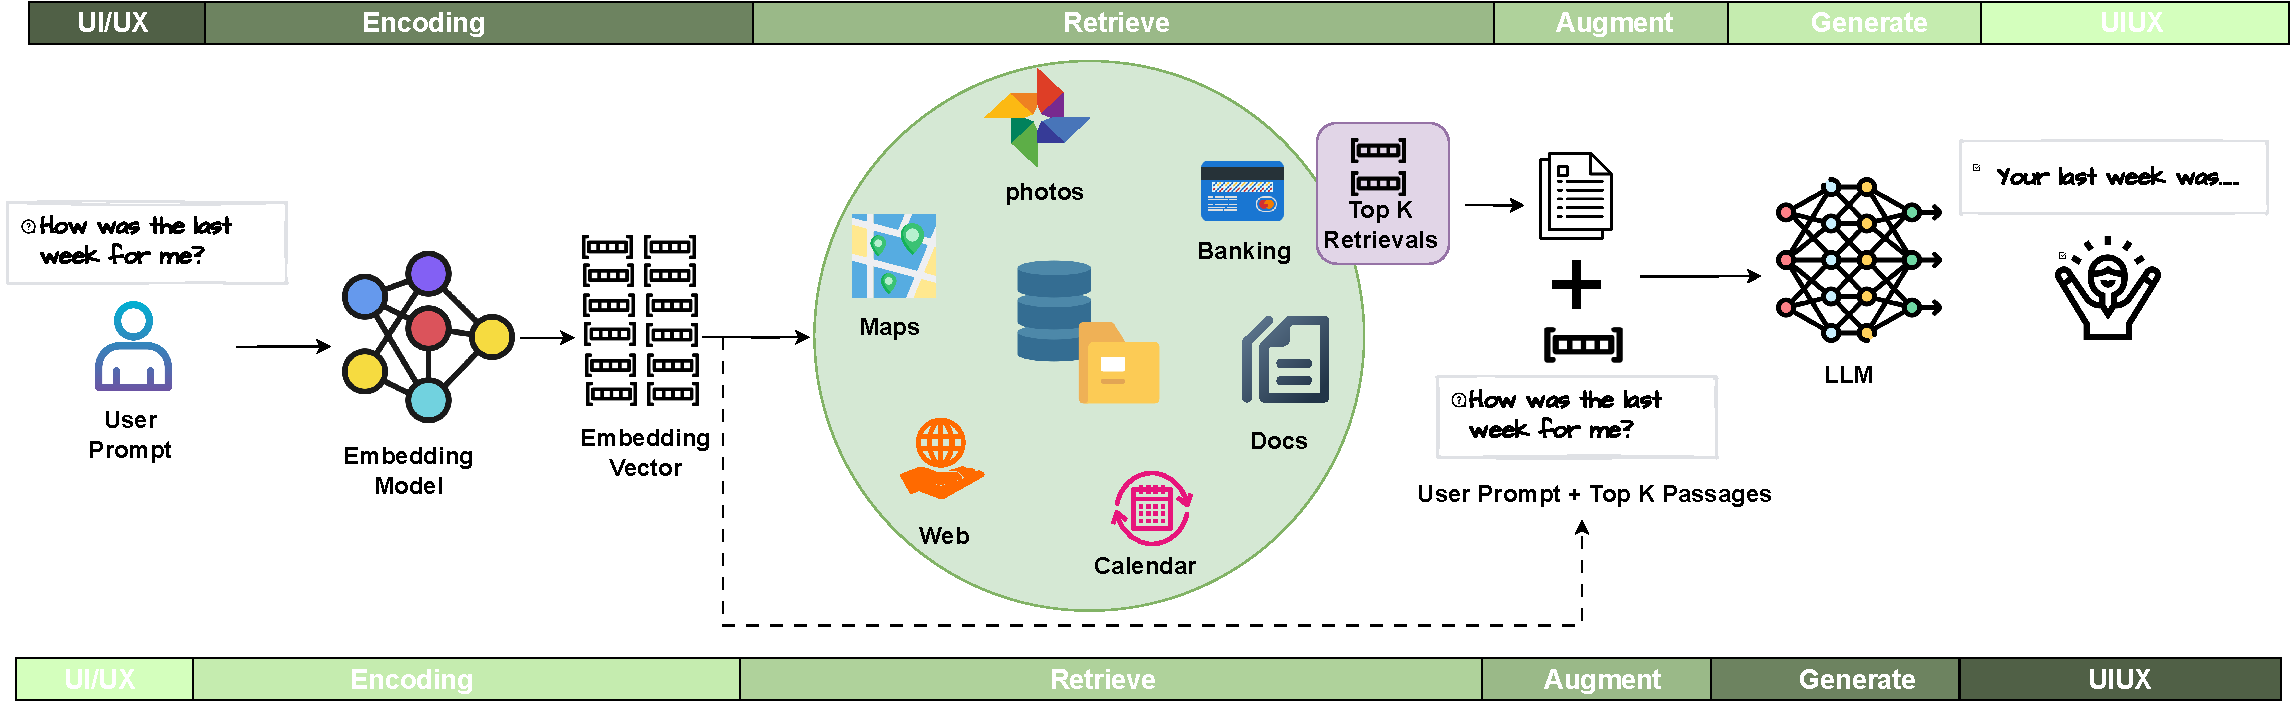
\includegraphics[width=0.75\linewidth]{Figs/RAGpipegrad.pdf}
% \caption{An illustration showing the end-to-end RAG 
% %\todo{suggestion: avoid using pipeline wording for describing application stages }
% pipeline. An user asks a query in his/her natural language which gets converted to higher dimensional embedding vector used to find \topk most similar elements from the local database.}
% \label{fig:RAG_background} 
% \vspace{-10pt}
% \end{figure*}
% %%%%%%%%%%
%%%%%%%%%%%%%%%%%%%%%%%%%%%%%%%%%%%%%%%%%%%%%%%%%%%%%%%%%%%%%%%%%%%%%%%%%%%%%%%%%%%%%%%%%%%

\section{Introduction}
\label{sec:intro}

Retrieval-Augmented Generation (RAG) combines compact language models with external knowledge retrieval, enabling personalized responses without embedding all knowledge in model parameters~\cite{rag_neurips}. This decoupling makes RAG attractive for edge deployment, where privacy constraints favor local processing and limited resources preclude large models. In particular, users increasingly prefer on-device or edge-based AI systems because sensitive personal data can remain local, reducing exposure to centralized cloud services and improving data privacy guarantees. At the same time, service providers and corporations are also motivated to shift inference workloads toward the edge, as offloading computation to user devices reduces datacenter resource consumption, lowers operational and energy costs, and decreases token-generation overhead associated with cloud-hosted inference.
However, deploying RAG efficiently on edge devices, which typically have a single GPU shared for all  tasks, remains challenging.
%\new{; \Cref{sec:BG:Scope} defines the personal-computing edge setting we target}.

% \begin{figure}
%     \centering
%     \includegraphics[width=0.8\linewidth]{Figs/RAGFlow.pdf}
%     \caption{Classical RAG Pipeline has structural hazard and CPU under-utilization. \design{} solves it with smart orchestration.}
%     \label{fig:maestroRAG}
%     \vspace{-10pt}
% \end{figure}

Existing RAG systems, as depicted in \Cref{fig:maestroRAG}, place both the encoding stage (converts queries to embeddings) and the generation stage (produces responses via an LLM) on the GPU~\cite{jin2024flashrag, jiang2024piperag}. On edge devices with single GPU, this creates a \emph{structural hazard}: encoding and generation cannot run concurrently, leading to pipeline bubbles and resource underutilization. Prior systems like FlashRAG~\cite{jin2024flashrag} and PipeRAG~\cite{jiang2024piperag} target datacenter deployments with abundant GPUs, while EdgeRAG~\cite{EdgeRAG} addresses edge scenarios but neither systematically optimize CPU--GPU coordination and nor perform smart orchestration.

In this paper, we present \textbf{MaestroRAG}, a fine-grained pipeline architecture for efficient RAG inference on edge devices. Our approach is grounded in workload characterization: we profile each RAG stage and find that \emph{encoding is compute-bound} and scales well on multicore CPUs, while \emph{retrieval is memory-bound} with diminishing returns from parallelism. Generation, in contrast, benefits from GPU acceleration. Based on these insights, MaestroRAG assigns encoding and retrieval to dedicated CPU cores while reserving the GPU exclusively for generation. This eliminates contention and enables true pipeline parallelism.

\begin{figure*}
    \centering
    % 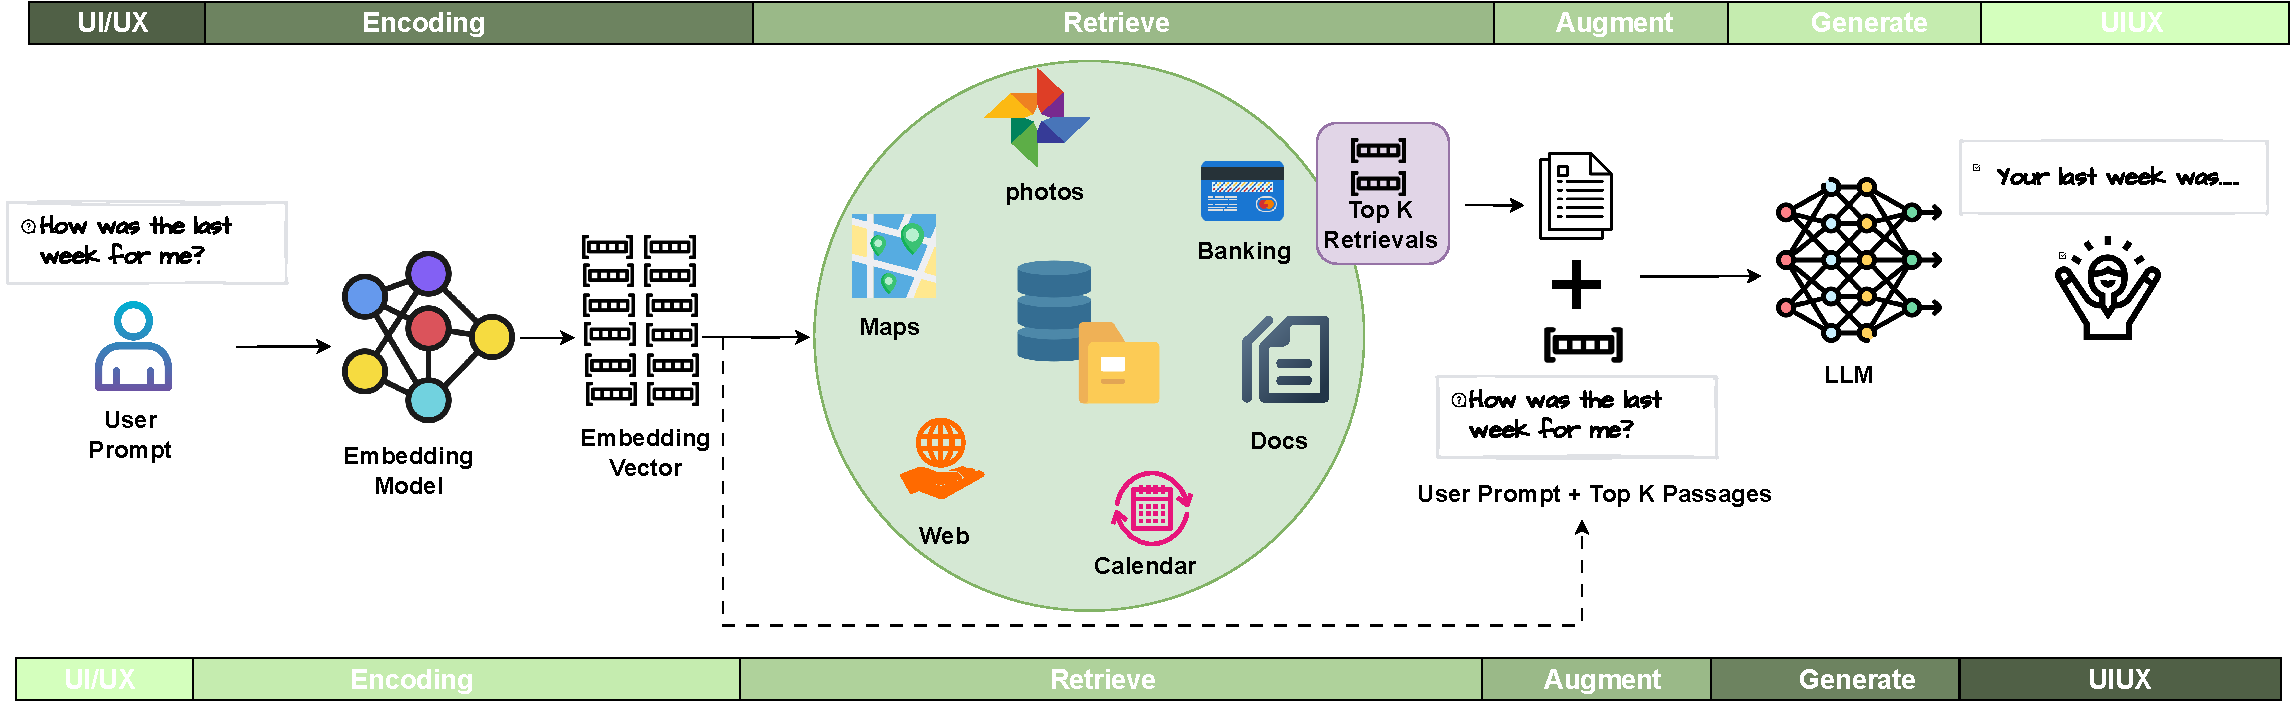
\includegraphics[width=0.8\linewidth]{Figs/RAGpipegrad.pdf}
    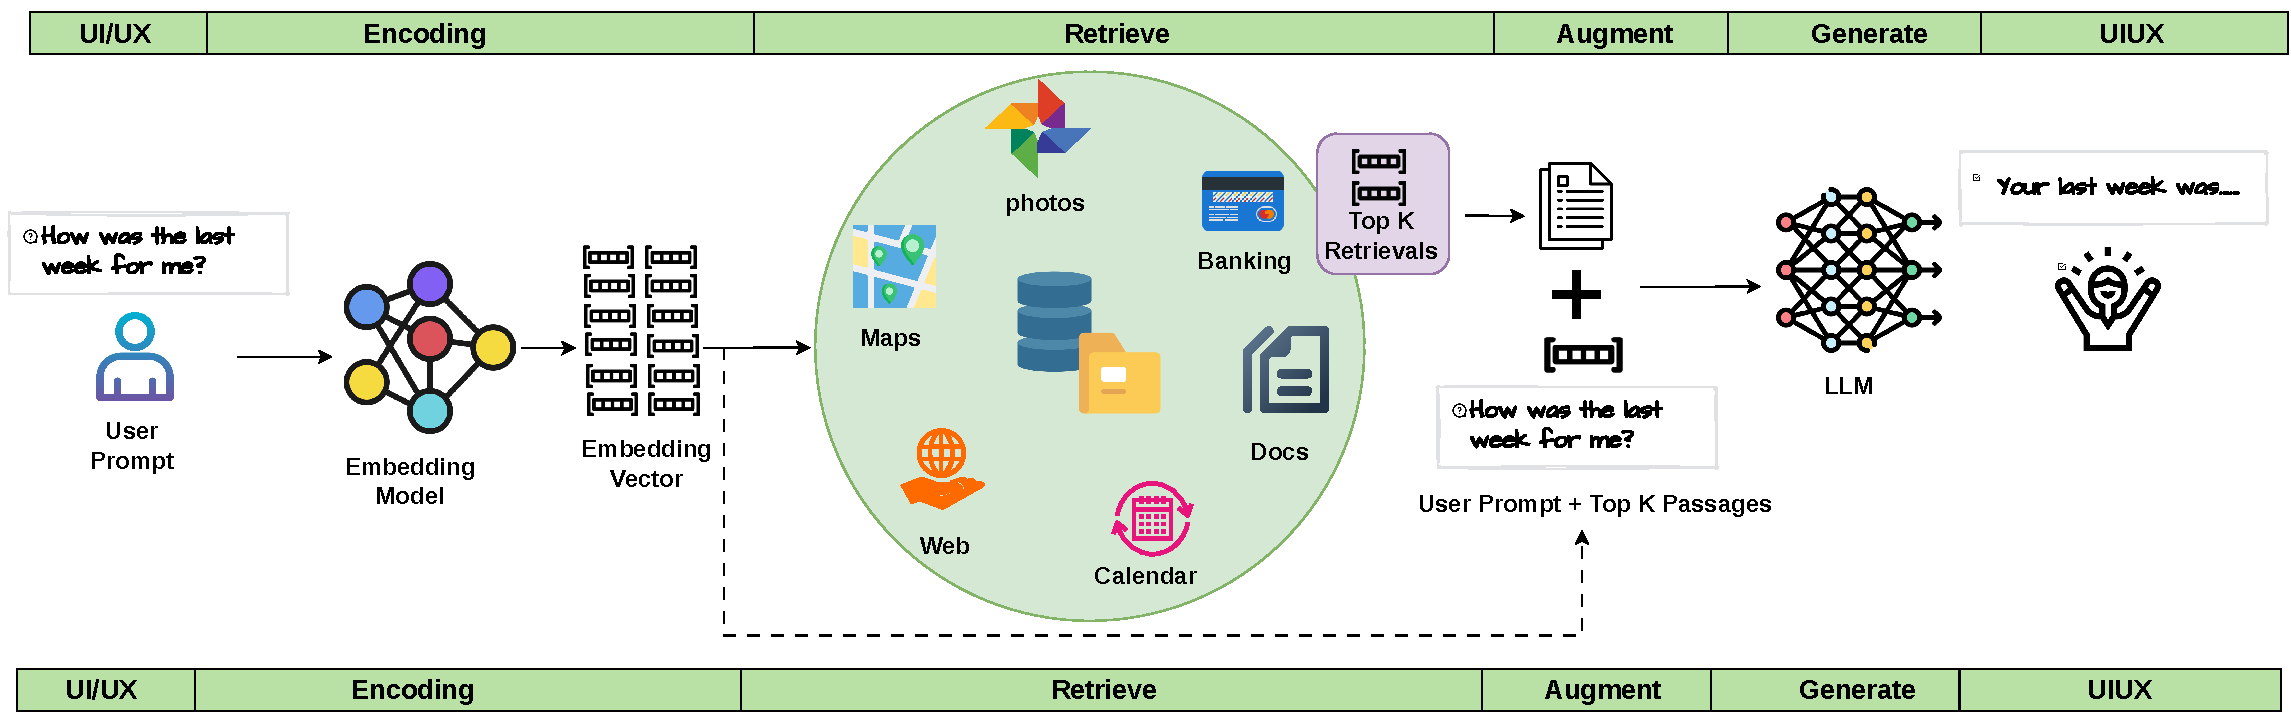
\includegraphics[width=0.8\linewidth]{Figs/ShepherdedMaestro.pdf}
    \caption{Classical RAG Pipeline has structural hazard and CPU under-utilization. \design{} solves it with smart orchestration.}
    \label{fig:maestroRAG}
    \vspace{-10pt}
\end{figure*}

We evaluated MaestroRAG on three platforms—NVIDIA RTX 4090, RTX 4080, and Jetson AGX Orin using realistic workloads derived from Azure traces and the Wikipedia corpus. Compared to state-of-the-art systems, MaestroRAG achieves a latency reduction of up to $12\times$, a performance improvement of $5.6\times$, and energy savings of $3\times$, while remaining agnostic to the choice of encoder and LLM. Our main {\bf contributions} in this work are:

% \begin{itemize}[leftmargin=1.5em, itemsep=2pt, topsep=3pt]
\noindent$\bullet$\textbf{Workload characterization} revealing that RAG encoding is compute-bound while retrieval is memory-bound, motivating heterogeneous CPU--GPU execution.

\noindent$\bullet$\textbf{A three-stage CPU--GPU pipeline} that eliminates structural hazards by partitioning encoding and retrieval across CPU cores while reserving the GPU for generation.

\noindent$\bullet$\textbf{Adaptive batching and multi-worker execution} to optimize for {\em both} latency-critical and throughput-critical workloads on resource-constrained devices.

\noindent$\bullet$\textbf{Comprehensive evaluation} on consumer-grade and embedded platforms, demonstrating significant improvements over FlashRAG~\cite{jin2024flashrag}, PipeRAG~\cite{jiang2024piperag}, and EdgeRAG~\cite{EdgeRAG}.
% \end{itemize}